\documentclass[11pt]{article}

\usepackage[utf8]{inputenc}
\usepackage[T1]{fontenc}
\usepackage{lmodern}
\usepackage[margin=0.9in]{geometry}
\usepackage{amsmath,amssymb,mathtools,bm}
\usepackage{booktabs,tabularx,array}
\usepackage{graphicx}
\usepackage{microtype}
\usepackage{xcolor}
\usepackage{enumitem}
\usepackage{hyperref}
\usepackage{cleveref}
\usepackage{tikz}
\usepackage{float}
\usepackage{placeins}
\usetikzlibrary{arrows.meta,positioning,calc,fit,shapes.geometric}

\hypersetup{
  colorlinks=true,
  linkcolor=blue!45!black,
  citecolor=blue!45!black,
  urlcolor=blue!45!black
}

\newcommand{\E}{\mathbb{E}}
\newcommand{\Var}{\operatorname{Var}}
\newcommand{\Cov}{\operatorname{Cov}}
\newcommand{\diag}{\operatorname{diag}}
\newcommand{\R}{\mathbb{R}}
\newcommand{\trans}{\mathsf T}
\newcommand{\norm}[1]{\left\lVert #1\right\rVert}
\newcommand{\given}{\,\middle|\,}
\newcommand{\conv}{\mathbin{*}}
\newcommand{\argmin}{\operatorname*{arg\,min}}
\newcommand{\argmax}{\operatorname*{arg\,max}}

\title{\textbf{From Patchwise Infomax to Spatiotemporal Convolutional ICA}\\
A Formal Proposal for Spatially Aware Neural-Activity Features in NeuRev}
\author{
Raul Valle \and Jos\'e C. Principe\\
Department of Electrical and Computer Engineering\\
University of Florida
}
\date{Working methods note --- July 29, 2026}

\begin{document}
\maketitle

\begin{abstract}
This note formalizes the proposal to evaluate an Infomax independent-component
objective on local image regions and extend it across space and time for
single-plane calcium imaging. The idea is valid, but three constructions must be
distinguished. \emph{Patch ICA} vectorizes fixed-size neighborhoods and treats
patches as repeated samples of one linear mixing model. \emph{Convolutional ICA}
constrains the analysis transform to a shared filter bank, producing
translation-equivariant component maps without patch boundaries.
\emph{Convolutive source separation} instead assumes that latent sources are
mixed through unknown temporal or spatial impulse responses. For the
single-channel Spon Ca Burst movie, none of these constructions guarantees
physical source recovery: pixels or time lags act as representation coordinates,
not independent sensors, and neural sources may coactivate. Nevertheless, a
noise-aware convolutional Infomax filter bank is a plausible feature extractor.
We propose a staged model that applies convolutional quiet whitening, learns
spatial filters under a tight-frame constraint, estimates marginal source scores
with noise-convolved Parzen densities, forms posterior-clean coefficient maps,
and reconstructs a structured residual through a declared synthesis operator.
A causal extension factorizes each space-time kernel into a spatial morphology
filter and a short temporal filter. The proposal is designed to discover
center-filled, annular, crowded-center, and crowded-annular activity while
retaining Raw Direct and Parzen Innovation as amplitude carriers. We derive the
classical and convolutional objectives, identify the underdetermined and
overcomplete boundaries, specify initialization and real-time constraints, and
preregister a sequence of falsifiable Spon Ca Burst experiments.
\end{abstract}

\section{Executive answer}

The proposed intuition is sound:
\begin{quote}
Use many local spatial or spatiotemporal neighborhoods as repeated observations,
and learn linear filters whose outputs are as statistically independent and
non-Gaussian as possible.
\end{quote}
The crucial refinement is that applying one ordinary ICA matrix to extracted
patch vectors is \emph{patchwise ICA}; it becomes convolutional ICA only when
the same learned filters are translated across the full field of view. Ball\'e
and Simoncelli formalized this distinction by replacing the dense ICA matrix
with convolutional Toeplitz blocks and constraining the filter bank in the
frequency domain \cite{balle2014cica}. Earlier work also showed that ICA applied
to natural movies can learn genuinely spatiotemporal filters
\cite{vanhateren1998stica}.

For NeuRev, the proposal is valuable for three reasons:
\begin{enumerate}[leftmargin=*]
\item spatial filters can represent a filled soma, an annular membrane, a
crowded soma, and a crowded annulus rather than scoring each pixel in isolation;
\item shared filters avoid arbitrary patch boundaries and use far fewer
parameters than a separate dense ICA matrix for every neighborhood;
\item short causal temporal filters can distinguish coherent calcium evolution
from framewise noise without discarding the absolute residual.
\end{enumerate}

The proposal also has a hard limitation. The movie has one fluorescence value
per pixel and time. It is not a conventional multichannel sensor array with
several simultaneous mixtures of the same physical sources. Patch coordinates
and temporal lags can be used as \emph{pseudo-channels}, but the recovered
components are learned local features unless stronger generative assumptions
are validated. The method should therefore be judged as a feature and
reconstruction model, not granted a physical-neuron interpretation by the ICA
objective alone.

\section{ICA refresher}

\subsection{Instantaneous linear ICA}

Classical noiseless ICA assumes observations
\begin{equation}
\bm x_n=A\bm s_n,\qquad
\bm x_n,\bm s_n\in\R^K,
\label{eq:ica-model}
\end{equation}
where $A$ is square and invertible and the entries of $\bm s_n$ are mutually
independent and non-Gaussian, with at most one Gaussian source. The demixer
$W\approx A^{-1}$ gives
\begin{equation}
\bm y_n=W\bm x_n.
\end{equation}
The solution is identifiable only up to permutation and nonzero scaling
(including sign). Bell and Sejnowski derived an information-maximization
algorithm whose nonlinear outputs maximize information transfer and thereby
reduce redundancy between the linear outputs \cite{bell1995infomax}.

Given source-density models $p_k$, the log-likelihood is
\begin{equation}
\mathcal L(W)
=
N\log|\det W|
+
\sum_{n=1}^{N}\sum_{k=1}^{K}
\log p_k(y_{nk}).
\label{eq:ica-likelihood}
\end{equation}
Let the negative marginal score be
\begin{equation}
\psi_k(y)=-\frac{\partial}{\partial y}\log p_k(y).
\end{equation}
One natural-gradient ascent convention is
\begin{equation}
\Delta W
=
\eta
\left[
I-\E\{\bm\psi(\bm y)\bm y^{\trans}\}
\right]W.
\label{eq:natural-gradient}
\end{equation}
Different publications use different score and ascent/descent signs; an
implementation must verify its convention by finite differences on a small
known mixture.

\subsection{Whitening and non-Gaussianity}

If
\begin{equation}
\bm z=Q(\bm x-\bm\mu),\qquad \Cov(\bm z)=I,
\end{equation}
then the remaining square demixer can be restricted to an orthogonal rotation
$U$, with $\bm y=U\bm z$. The determinant contribution is constant, so ICA can
be viewed as minimizing marginal entropies or maximizing non-Gaussianity subject
to decorrelation. FastICA uses fixed-point iterations with tractable contrast
functions such as $\log\cosh(y)$ \cite{hyvarinen1999fastica}. This explains a
useful practical summary:
\begin{quote}
PCA/whitening removes second-order dependence; ICA chooses a rotation using
higher-order statistics.
\end{quote}

\subsection{What independence means in an image movie}

There are two common matrix arrangements for a movie
$X\in\R^{T\times P}$:
\begin{align}
X&=CS^{\trans}
&&\text{independent temporal coefficients or traces},\\
X&=AC
&&\text{independent spatial maps}.
\end{align}
The choice is not cosmetic. Spatial ICA assumes spatial maps are independent
while allowing temporal dependence; temporal ICA assumes traces are independent
while allowing spatial overlap. Neural sources can be spatially overlapping and
temporally coactive, so either assumption can fail
\cite{calhoun2001spatialtemporal}. For calcium imaging, PCA followed by ICA has
historically been useful for cellular signal extraction
\cite{mukamel2009calcium}, but constrained nonnegative matrix factorization
often handles overlapping nonnegative footprints and calcium dynamics more
faithfully \cite{pnevmatikakis2016cnmf}.

\section{Three related models that should not be conflated}

\subsection{Model A: patchwise ICA}

Let $P_{\bm r}$ extract an $h\times w$ patch centered at spatial location
$\bm r$. For frame $t$,
\begin{equation}
\bm x_{t,\bm r}
=
\operatorname{vec}\!\left(P_{\bm r}R_t\right)
\in\R^{hw}.
\label{eq:patch-vector}
\end{equation}
All selected $(t,\bm r)$ pairs become samples of one patch distribution:
\begin{equation}
\bm y_{t,\bm r}
=
WQ(\bm x_{t,\bm r}-\bm\mu).
\label{eq:patch-ica}
\end{equation}
The Infomax objective in \cref{eq:ica-likelihood} is then summed over patches.
It seeks independence among entries of $\bm y$ \emph{over the patch ensemble};
it does not seek independence between neighboring patches.

Patch ICA is the simplest literal version of the proposed idea. It can learn
localized edge, center-surround, and texture filters
\cite{bellsejnowski1997edges}. It also has weaknesses:
\begin{itemize}[leftmargin=*]
\item a feature at the center and the same feature near an edge occupy different
coordinates;
\item nonoverlapping patches create blocking artifacts;
\item overlapping reconstruction requires a declared window and normalization;
\item a dense $hw\times hw$ transform grows quickly with patch size;
\item pixels within a patch are treated as mixture coordinates, not sensors with
known physical mixing diversity.
\end{itemize}

\subsection{Model B: convolutional ICA as an analysis filter bank}

Convolutional ICA shares filters across all locations. After stationary
whitening,
\begin{equation}
Z_t=q\conv (R_t-\mu_q),
\end{equation}
the $k$th component map is
\begin{equation}
Y_{k,t}(\bm r)
=
(b_k\conv Z_t)(\bm r).
\label{eq:spatial-cica}
\end{equation}
The dense matrix associated with each convolution is Toeplitz. Translation of
an input feature produces the corresponding translation of its component map,
apart from the boundary convention.

For an undecimated Parseval-like analysis bank, the isometry condition is
\begin{equation}
\sum_{k=1}^{K}B_k^{\trans}B_k=I,
\label{eq:isometry-spatial}
\end{equation}
or, under a circulant approximation,
\begin{equation}
\forall\bm\omega:\qquad
\sum_{k=1}^{K}
|\widetilde b_k(\bm\omega)|^2=1.
\label{eq:fourier-tight}
\end{equation}
Ball\'e and Simoncelli alternate a FastICA-like marginal update with
frequency-domain enforcement of this constraint
\cite{balle2014cica}. The model avoids patch boundaries and reduces the number
of learned parameters. Critically sampled versions can be square and closer to
classical ICA; dense undecimated versions are overcomplete and require more
care in interpreting ``independence.''

\subsection{Model C: a generative convolutional source model}

A different construction assumes that the movie is synthesized from latent
activation maps:
\begin{equation}
R_t
=
\sum_{k=1}^{K}d_k\conv A_{k,t}
+N_t.
\label{eq:conv-generative}
\end{equation}
Here $d_k$ is a spatial atom or footprint prototype, $A_{k,t}$ is a sparse
activation map, and $N_t$ is noise. If $K$ is large, this is more naturally
called convolutional sparse coding than square ICA
\cite{bristow2013csc}. It is appealing for neuron morphology because one atom
can occur at many locations, but physical neurons are not exact translations
of a small number of templates. A hybrid model can use convolutional ICA to
learn the analysis filters and an explicit synthesis operator to reconstruct
and audit the representation.

\subsection{Convolutional versus convolutive ICA}

The terminology is easy to confuse:
\begin{itemize}[leftmargin=*]
\item \emph{convolutional ICA} in image representation usually means a
translation-shared analysis filter bank;
\item \emph{convolutive ICA} in blind source separation usually means sources
are mixed through unknown impulse responses, often over time.
\end{itemize}
Bell and Sejnowski included delayed filters and blind-deconvolution examples
\cite{bell1995infomax}. NeuRev's proposed three-dimensional kernels borrow from
both ideas, but the scientific goal is a local space-time representation rather
than recovery from several physical microphones or electrodes.

\section{Proposed NeuRev model}

\subsection{Input and role in the existing pipeline}

The initial experiment should use the signed, amplitude-preserving Parzen
Innovation residual
\begin{equation}
R_t=X_t-\widehat B_t
\end{equation}
and retain Raw Direct as a parallel frozen lane. Quiet frames define per-pixel
median and robust scale:
\begin{equation}
Z_t(p)
=
\frac{R_t(p)-\mu_q(p)}
{\max\{\sigma_q(p),\sigma_{\min}\}}.
\label{eq:quiet-standard}
\end{equation}
This standardization prevents permanently noisy pixels from dominating filter
learning. It should be followed by a bounded stationary convolutional whitening
filter, not a full dense whitening matrix over the field.

\begin{figure}[H]
\centering
\resizebox{\textwidth}{!}{%
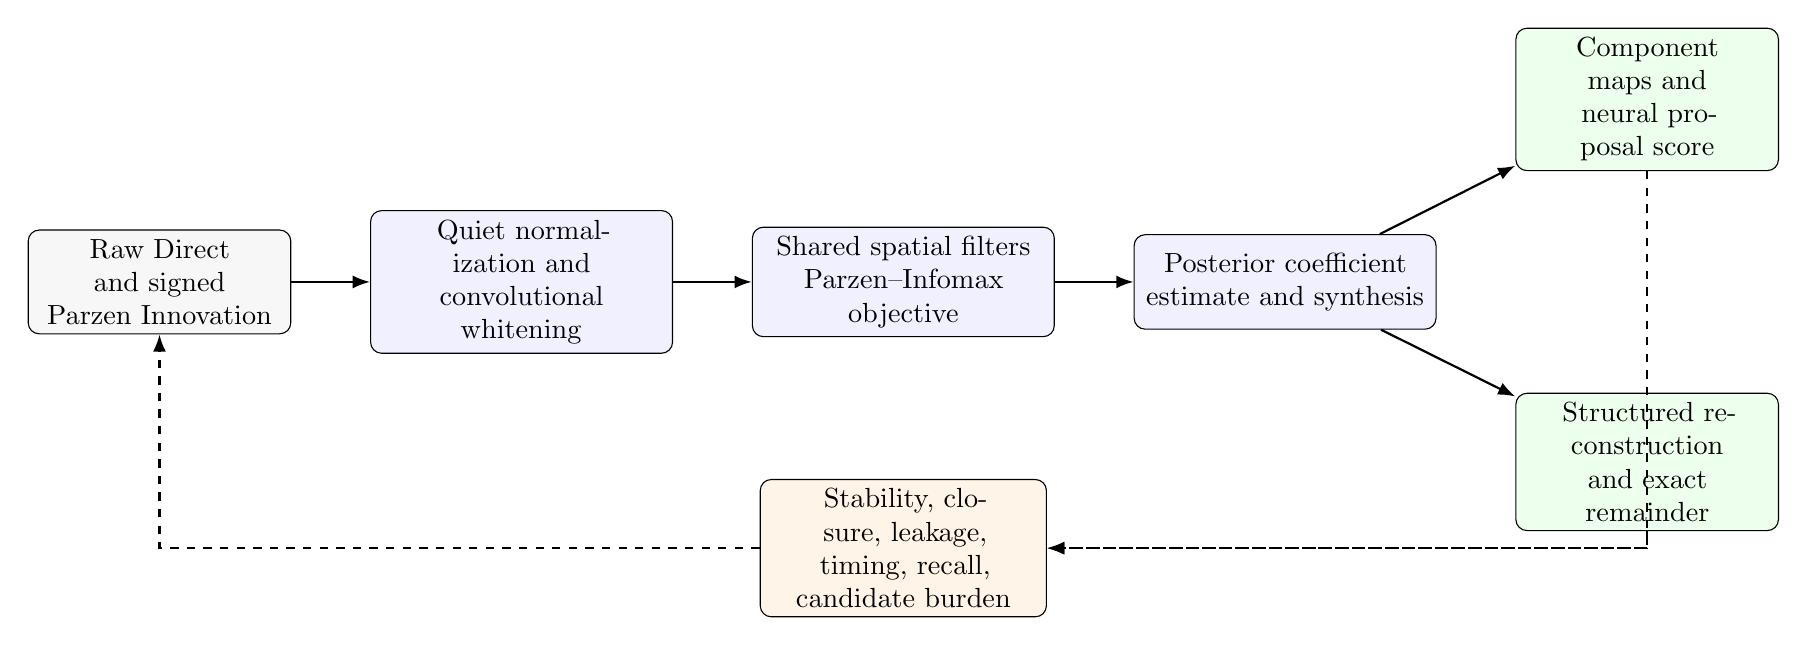
\begin{tikzpicture}[
  node distance=8mm and 10mm,
  box/.style={draw, rounded corners, align=center, minimum height=11mm,
              text width=31mm, fill=black!3},
  stage/.style={draw, rounded corners, align=center, minimum height=12mm,
                text width=36mm, fill=blue!6},
  output/.style={draw, rounded corners, align=center, minimum height=10mm,
                 text width=31mm, fill=green!7},
  guard/.style={draw, rounded corners, align=center, minimum height=10mm,
                text width=34mm, fill=orange!9},
  arrow/.style={-{Latex[length=2.2mm]}, thick}
]
\node[box] (input) {Raw Direct and signed\\Parzen Innovation};
\node[stage, right=of input] (white) {Quiet normalization and\\convolutional whitening};
\node[stage, right=of white] (cica) {Shared spatial filters\\Parzen--Infomax objective};
\node[stage, right=of cica] (post) {Posterior coefficient\\estimate and synthesis};
\node[output, above right=8mm and 10mm of post] (maps) {Component maps and\\neural proposal score};
\node[output, below right=8mm and 10mm of post] (recon) {Structured reconstruction\\and exact remainder};
\node[guard, below=18mm of cica] (audit) {Stability, closure, leakage,\\timing, recall, candidate burden};

\draw[arrow] (input) -- (white);
\draw[arrow] (white) -- (cica);
\draw[arrow] (cica) -- (post);
\draw[arrow] (post) -- (maps);
\draw[arrow] (post) -- (recon);
\draw[arrow, dashed] (maps) |- (audit.east);
\draw[arrow, dashed] (recon) |- (audit.east);
\draw[arrow, dashed] (audit.west) -| (input.south);
\end{tikzpicture}%
}
\caption{The proposed model is an auditable feature branch. It does not replace
the amplitude carriers unless it passes reconstruction, event-preservation, and
detection gates.}
\label{fig:proposed-pipeline}
\end{figure}

\subsection{Noise-aware Parzen marginals}

For a component coefficient
\begin{equation}
y_{k}=a_k+\eta_k,\qquad
\eta_k\sim\mathcal N(0,\nu_k^2),
\end{equation}
represent the latent clean marginal using a Gaussian Parzen dictionary:
\begin{equation}
\widehat p_{a_k}(a)
=
\frac1M\sum_{m=1}^{M}
\mathcal N(a;c_{km},h_k^2).
\end{equation}
The observed marginal is the convolution
\begin{equation}
\widehat p_{y_k}(y)
=
\frac1M\sum_{m=1}^{M}
\mathcal N
\left(y;c_{km},h_k^2+\nu_k^2\right).
\label{eq:noisy-parzen}
\end{equation}
The projected noise variance can be measured from quiet responses or estimated
from a quiet noise spectrum:
\begin{equation}
\nu_k^2
\approx
\E_{t\in\mathcal Q,\bm r}Y_{k,t}(\bm r)^2
\quad\text{or}\quad
\int |\widetilde b_k(\bm\omega)|^2
S_N(\bm\omega)\,d\bm\omega.
\end{equation}

Define responsibilities
\begin{equation}
\alpha_{km}(y)
=
\frac{
\mathcal N(y;c_{km},h_k^2+\nu_k^2)
}{
\sum_{\ell}
\mathcal N(y;c_{k\ell},h_k^2+\nu_k^2)
}.
\end{equation}
The negative score used in \cref{eq:natural-gradient} is
\begin{equation}
\psi_k(y)
=
\frac{
y-\sum_m\alpha_{km}(y)c_{km}
}{
h_k^2+\nu_k^2
}.
\label{eq:parzen-score}
\end{equation}
The posterior clean coefficient has analytic mean
\begin{equation}
\widehat a_k(y)
=
\sum_m\alpha_{km}(y)
\frac{
\nu_k^2c_{km}+h_k^2y
}{
h_k^2+\nu_k^2
}.
\label{eq:parzen-posterior}
\end{equation}
This preserves the distinction between learning a demixing direction and
estimating a clean coefficient after demixing.

\subsection{A practical objective}

For dense overcomplete filters, the exact square-ICA determinant is unavailable.
The proposed training objective should state that it is a constrained
Infomax-inspired filter-bank objective:
\begin{align}
\mathcal J
={}&
\frac{1}{|\mathcal I|}
\sum_{(t,\bm r)\in\mathcal I}
\sum_{k=1}^{K}
\left[
-\log\widehat p_{y_k}
\left(Y_{k,t}(\bm r)\right)
\right]
\nonumber\\
&+
\lambda_{\mathrm{tight}}
\sum_{\bm\omega}
\left(
\sum_k|\widetilde b_k(\bm\omega)|^2-1
\right)^2
\nonumber\\
&+
\lambda_{\mathrm{dep}}
\mathcal D_{\mathrm{dep}}
\left(\{Y_k\}_{k=1}^{K}\right)
+
\lambda_{\mathrm{rec}}
\mathcal L_{\mathrm{rec}}.
\label{eq:working-objective}
\end{align}
The first term is a marginal entropy/coding term using
\cref{eq:noisy-parzen}; the second prevents collapse and enforces approximate
coverage of the frequency plane; the third is a bounded pairwise
higher-order-dependence estimate, such as a Cauchy--Schwarz or kernel
dependence criterion; and the fourth verifies that the chosen synthesis
operator can reconstruct the standardized residual. An overcomplete bank must
not be forced to have identity output covariance: its output covariance is
rank deficient by construction. For a critically sampled square bank, the
dependence and determinant treatment can follow classical ICA more directly.
For an undecimated bank, \cref{eq:working-objective} is a transparent hybrid
rather than a claim of exact classical ICA.

Dictionary centers cannot be allowed to follow the outputs without constraint,
because the density and filters could co-adapt to a trivial representation.
Use a bounded half-zero dictionary, slow posterior-center updates, bandwidth
bounds, a frozen quiet noise estimate, and alternating rather than simultaneous
updates.

\subsection{Analysis, posterior shrinkage, and synthesis}

The analysis coefficients are
\begin{equation}
Y_{k,t}=b_k\conv Z_t.
\end{equation}
Apply \cref{eq:parzen-posterior} pointwise:
\begin{equation}
\widehat A_{k,t}(\bm r)
=
\widehat a_k\!\left(Y_{k,t}(\bm r)\right).
\end{equation}
If the analysis bank is Parseval tight, an initial synthesis is the adjoint:
\begin{equation}
\widehat Z_t
=
\sum_{k=1}^{K}
\widetilde b_k\conv \widehat A_{k,t},
\label{eq:tight-synthesis}
\end{equation}
where $\widetilde b_k$ is the spatially reversed filter. Otherwise, use a
declared dual filter bank or solve a bounded least-squares reconstruction.
Always retain the exact unresolved remainder
\begin{equation}
\widehat U_t=Z_t-\widehat Z_t.
\label{eq:exact-remainder}
\end{equation}
Recognizable neurons or propagating activity in $\widehat U$ indicate
over-shrinkage even when the coefficient objective improves. This channel must
not be called measurement noise unless separate residual-validity tests support
that interpretation.

\subsection{Why this may represent the four observed morphologies}

The learned filters are not told which morphology is correct. Their shared
support nevertheless permits filters that respond to:
\begin{enumerate}[leftmargin=*]
\item a positive center with suppressive surroundings;
\item an annulus with a dark center;
\item a center conditioned on illuminated neighbors;
\item an annulus conditioned on illuminated neighbors.
\end{enumerate}
A single linear filter cannot make all four cases independent. Use small
\emph{groups} of related filters, for example center, annular, broad-neighbor,
and edge/artifact responses. Independence is then encouraged between group
energies rather than between every member:
\begin{equation}
G_{g,t}(\bm r)
=
\left[
\sum_{k\in\mathcal G_g}
Y_{k,t}(\bm r)^2+\epsilon
\right]^{1/2}.
\label{eq:group-energy}
\end{equation}
This is closer to independent-subspace or topographic ICA, which explicitly
permits structured dependence within local component groups
\cite{hyvarinen2001tica}. It also reduces the risk that correlated center and
membrane responses are forced into unstable arbitrary rotations.

\section{Temporal extension}

\subsection{Patchwise spatiotemporal ICA}

The direct extension of \cref{eq:patch-vector} stacks $L$ frames:
\begin{equation}
\bm x_{t,\bm r}
=
\operatorname{vec}
\left(
\left\{
P_{\bm r}R_{t-\tau}
\right\}_{\tau=0}^{L-1}
\right)
\in\R^{Lhw}.
\label{eq:st-patch}
\end{equation}
Ordinary ICA on these vectors can learn moving or evolving space-time patterns,
as demonstrated on natural image sequences
\cite{vanhateren1998stica}. Its parameter count and whitening cost grow with
$Lhw$, so it is best used as a small scientific reference.

\subsection{Three-dimensional convolutional ICA}

A causal space-time filter produces
\begin{equation}
Y_{k,t}(\bm r)
=
\sum_{\tau=0}^{L-1}
\sum_{\bm u\in\Omega}
b_k(\tau,\bm u)
Z_{t-\tau}(\bm r-\bm u).
\label{eq:3d-cica}
\end{equation}
No future frame appears. The three-dimensional tight-frame analogue is
\begin{equation}
\forall(\omega_t,\bm\omega):
\quad
\sum_k
|\widetilde b_k(\omega_t,\bm\omega)|^2
\approx1.
\end{equation}
This model can learn joint morphology and kinetics, but it is substantially
harder to identify and audit. Neural events also share calcium dynamics, so
strict temporal independence may split amplitude, onset, and decay into
artificial components.

\subsection{Recommended factorized causal model}

Begin with
\begin{equation}
b_k(\tau,\bm u)=h_k(\tau)g_k(\bm u),
\label{eq:factorized-kernel}
\end{equation}
so that
\begin{equation}
Y_{k,t}
=
h_k\conv_t
\left(g_k\conv_{xy}Z\right)_t.
\end{equation}
This separates two interpretable questions:
\begin{itemize}[leftmargin=*]
\item what local spatial morphology does $g_k$ recognize?
\item what short causal evolution does $h_k$ retain or reject?
\end{itemize}
Initialize temporal filters as identity, short smoothers, onset differences,
and calcium-like decays. Permit at most a short lookback initially. A five-frame
kernel spans 100 ms at the Spon Ca Burst 20 ms frame period.

\section{Initialization and optimization}

\subsection{Spatial initialization}

Random orthogonal initialization is a useful control but not the only sensible
starting point. The proposed warm start contains:
\begin{itemize}[leftmargin=*]
\item an identity/low-pass carrier;
\item Gaussian center-surround filters at two radii;
\item annular filters at two radii;
\item broad-neighbor and oriented edge filters;
\item high-frequency residual filters completing the tight frame.
\end{itemize}
These are initial coordinates, not fixed definitions of a neuron. Project the
bank onto the frequency-domain constraint before the first update. Compare with
at least three seeded random banks to determine whether the learned result is
an initialization artifact.

\subsection{Optimization schedule}

A safe alternating schedule is:
\begin{enumerate}[leftmargin=*]
\item freeze quiet center, scale, noise spectrum, and output contract;
\item fit or freeze convolutional whitening;
\item update filters for one bounded epoch with the Parzen dictionary frozen;
\item project onto the tight-frame constraint and clip the update norm;
\item update posterior dictionary centers slowly from bounded clean-coefficient
samples;
\item evaluate objective direction, closure, filter drift, and held-out
stability;
\item stop if any numerical or scientific gate fails.
\end{enumerate}
Use a low learning rate because the hand-designed bank is a meaningful
coordinate system. An initial range of $10^{-5}$ to $3\times10^{-4}$ is
appropriate for natural-gradient tuning, but the accepted value must be chosen
by update norms and held-out stability rather than training loss alone.

\subsection{Avoiding degenerate solutions}

Reject or reinitialize a fit when any of the following occurs:
\begin{itemize}[leftmargin=*]
\item one filter receives nearly all response energy;
\item two filters become shifted or signed duplicates without a declared group;
\item a frequency band is uncovered or excessively amplified;
\item the synthesis condition number exceeds its cap;
\item dictionary bandwidth collapses or centers chase outliers;
\item quiet coefficients become less white or more structured;
\item the reconstructed signal loses labeled amplitude or timing;
\item results are unstable under seeds, patch phases, or held-out bursts.
\end{itemize}

\section{Real-time interpretation}

With frozen filters, the spatial model is a conventional small-kernel
convolution followed by lookup-table posterior shrinkage and synthesis. This is
compatible with real-time GPU inference. Online \emph{learning} is a separate
question and should occur at a slower timescale.

\begin{table}[H]
\centering
\caption{Two-timescale deployment contract.}
\begin{tabularx}{\textwidth}{@{}p{0.18\textwidth}X X@{}}
\toprule
 & Fast frame path & Slow adaptation path\\
\midrule
Operations &
quiet normalization, causal convolution, posterior lookup, component score,
late fusion &
noise-scale update, dictionary maintenance, bounded filter update,
stability audit\\
Labels used &
none &
none during unsupervised fitting; held labels only for external evaluation\\
Failure action &
fall back to frozen Raw Direct/Parzen lane &
reject update and keep last accepted filters\\
Timing target &
p95 below 20 ms per frame &
bounded background task with no acquisition deadline\\
\bottomrule
\end{tabularx}
\end{table}

Do not call an offline 560-frame patch SVD or batch ICA ``real-time'' merely
because average throughput is fast. The causal model may depend only on current
and past state, must bound memory, and must declare its p50/p95/p99 latency.
Online calcium-analysis systems demonstrate that causal source tracking is
feasible, but they maintain explicit source footprints and temporal state
\cite{giovannucci2017onacid,friedrich2017oasis}.

\section{Experimental program}

\subsection{Primary question}

Does a shared spatial or spatiotemporal Infomax filter bank add useful,
shape-aware evidence beyond unfiltered Parzen Innovation and Raw Direct without
destroying event amplitude, waveform, or timing?

\subsection{Sequential model ladder}

\begin{table}[H]
\centering
\small
\caption{Each stage advances only if it improves a declared audit dimension
without crossing preservation or stability gates.}
\begin{tabularx}{\textwidth}{@{}p{0.08\textwidth}p{0.27\textwidth}X@{}}
\toprule
Stage & Model & Purpose\\
\midrule
C0 & Existing frozen lanes &
Raw Direct, Parzen Innovation, temporal gate, local PCA, noise-normalized PCA,
and local PCA/ICA/Parzen anchors.\\
C1 & Patch FastICA &
Literal test of Infomax on vectorized spatial patches; establishes whether
higher-order spatial rotation adds value beyond PCA.\\
C2 & Spatial convolutional FastICA &
Tests weight sharing and removal of patch boundaries using a conventional
contrast.\\
C3 & Spatial convolutional Parzen-Infomax &
Replaces the fixed contrast with the noise-aware score and posterior estimate.\\
C4 & Grouped spatial model &
Allows dependent center, annular, neighbor, and artifact filters within
independent subspaces.\\
C5 & Factorized causal space-time model &
Adds short temporal filters after the accepted spatial bank.\\
C6 & Full three-dimensional model &
Runs only if C5 is stable and morphology--kinetics interactions remain
unexplained.\\
\bottomrule
\end{tabularx}
\end{table}

\subsection{Initial bounded grid}

The first breadth screen should remain small:
\begin{itemize}[leftmargin=*]
\item spatial support: $9$, $13$, and $17$ pixels;
\item component count: $8$, $16$, and $32$;
\item dense versus critically sampled scientific reference;
\item fixed $\log\cosh$ versus noisy-Parzen marginal;
\item random versus morphology warm start;
\item temporal lookback for C5: $3$, $5$, and $9$ frames.
\end{itemize}
Do not cross all values blindly. First choose a spatial support and component
count using C1--C2 stability, then test the marginal objective, then add time.
Use successive halving based on hard numerical gates followed by scientific
preservation gates.

\subsection{Data split}

The current Spon Ca Burst labels cover four bursts in one small associated
sequence. Any fit on all 560 frames is exploratory and transductive. For the
strongest available internal check:
\begin{enumerate}[leftmargin=*]
\item train the unsupervised model on the quiet interval and three burst
contexts;
\item freeze all filters, dictionaries, scales, and thresholds;
\item evaluate the fourth burst;
\item rotate over four held bursts;
\item repeat across at least three initializations.
\end{enumerate}
Future claims of generalization require held-out fish or sessions.

\subsection{Semi-synthetic morphology test}

Inject exact sources into real quiet residuals:
\begin{equation}
Z^{\mathrm{obs}}=Z^{\mathrm{quiet}}+S^{\mathrm{inject}}.
\end{equation}
Use filled, annular, crowded-filled, and crowded-annular sources separately at
several amplitudes. Report each morphology independently rather than only one
aggregate correlation. Measure:
\begin{itemize}[leftmargin=*]
\item source NMSE and correlation;
\item footprint IoU and centroid error;
\item peak/area retention and onset/peak timing;
\item leakage of the injected truth into the exact remainder;
\item false structured responses outside the injected support.
\end{itemize}

\subsection{Real sparse-label evaluation}

Retain the current sparse-label contract:
\begin{itemize}[leftmargin=*]
\item quiet-calibrated mean and pooled known-label recall;
\item fixed-budget recall with the budget stated per burst;
\item candidate burden and FROC;
\item amplitude, area, waveform, onset, peak, and duration preservation;
\item recurrence and seed stability;
\item visual signal/remainder review.
\end{itemize}
Unmatched candidates remain unknown, not false positives. Precision requires an
exhaustively annotated subset.

\subsection{Representation diagnostics}

An ICA-like method should also report what its own objective claims to improve:
\begin{itemize}[leftmargin=*]
\item covariance error before and after whitening;
\item tight-frame error over spatial or space-time frequency;
\item marginal kurtosis, negentropy surrogate, and Parzen log-density;
\item pairwise residual dependence or held-out multi-information proxy;
\item filter localization, bandwidth, duplicate similarity, and seed matching;
\item analysis/synthesis condition number and exact closure;
\item quiet residual autocorrelation and spatial spectrum.
\end{itemize}
Objective improvement without downstream or reconstruction improvement is a
representation result, not a neural-detection success.

\section{Falsifiable hypotheses and stop rules}

\paragraph{H1: spatial sharing helps.}
C2 should reduce patch-phase sensitivity and improve stability relative to C1.
If it does not, convolutional sharing is not earning its added complexity.

\paragraph{H2: Parzen scoring helps under noncanonical morphology.}
C3 should improve at least one morphology-specific semi-synthetic result and
held-burst detection relative to C2 without increasing signal leakage. If it
only lowers the training entropy surrogate, stop.

\paragraph{H3: grouped components handle coactivation.}
C4 should improve crowded-source recovery or seed stability. If groups merely
duplicate filters, return to C3.

\paragraph{H4: short causal memory suppresses noise without timing damage.}
C5 should improve quiet attenuation or candidate ranking while keeping median
peak error at most one frame and peak/area retention above a predeclared bound.
If it reproduces the earlier Kalman/Haar timing shift, do not run C6.

\paragraph{Global stop rule.}
Do not advance any branch that underperforms both Raw Direct and the matching
unfiltered Parzen input on held-burst detection while also worsening
semi-synthetic recovery or labeled event preservation.

\section{Expected outcomes and honest interpretation}

There are four plausible outcomes:
\begin{enumerate}[leftmargin=*]
\item \textbf{Useful filters and better detection.} Convolutional ICA becomes an
accepted proposal feature, still fused with amplitude.
\item \textbf{Useful morphology but no detector gain.} The filters become
diagnostic visual channels or initialization for a supervised proposal model.
\item \textbf{Stable denoising but source leakage.} Retain the method only for
visualization; do not call the reconstruction neural signal.
\item \textbf{Edge/derivative rediscovery.} The result confirms that the
Infomax objective prefers motion/change statistics in this dataset. Return to
explicit neuron footprints and trace-level models.
\end{enumerate}

The fourth outcome is scientifically meaningful. Natural-image ICA often
learns localized oriented filters \cite{bellsejnowski1997edges}, and NeuRev's
adjacent-frame ICA already rediscovered a derivative direction. The proposed
experiment is valuable precisely because it can reveal whether spatial
morphology changes that outcome.

\section{Recommendation}

Implement C1 and C2 first. Use the existing local PCA/ICA code only as a
reference, then add one reusable convolutional filter-bank module with explicit
analysis, constraint projection, synthesis, and serialization boundaries.
Initially:
\begin{itemize}[leftmargin=*]
\item input the signed Parzen Innovation residual;
\item use 13-pixel spatial support and 16 filters;
\item compare a morphology warm start with three random seeds;
\item use a fixed FastICA contrast before adding the Parzen dictionary;
\item write filter mosaics, component-map TIFFs, structured reconstruction,
and exact remainder;
\item evaluate held-burst stability and the four morphology fixtures;
\item keep labels outside unsupervised fitting.
\end{itemize}

Only after that reference is stable should NeuRev substitute the noisy-Parzen
score, group related filters, and add a three- or five-frame causal temporal
kernel. This order tests the central idea without making convolution, Parzen
density estimation, temporal memory, overcompleteness, and neural
classification fail simultaneously.

\section{Questions to take to the group}

\begin{enumerate}[leftmargin=*]
\item Should the first scientific target be an invertible critically sampled
filter bank or a dense shift-equivariant proposal bank?
\item Is independence more plausible between spatial component maps, temporal
traces, or groups of morphology filters in this preparation?
\item What cell diameters in pixels define the biologically meaningful spatial
support?
\item Is 20--100 ms of causal memory sufficient to reject frame noise while
preserving observed propagation?
\item Should annular and filled responses be treated as one independent
subspace rather than competing independent components?
\item Which exhaustively annotated tiles can support precision-oriented model
selection?
\end{enumerate}

\appendix
\section{Compact derivation of the patch objective}

For patch samples $\bm x_i$ and invertible $W$, change of variables gives
\begin{equation}
p_{\bm x}(\bm x_i)
=
|\det W|
\prod_k p_k(\bm w_k^{\trans}\bm x_i).
\end{equation}
Summing logarithms gives \cref{eq:ica-likelihood}. Differentiating,
\begin{equation}
\nabla_W\mathcal L
=
NW^{-\trans}
-
\sum_i
\bm\psi(\bm y_i)\bm x_i^{\trans}.
\end{equation}
Right multiplication by $W^{\trans}W/N$ yields the relative/natural-gradient
form in \cref{eq:natural-gradient}. Replacing sample index $i$ with patch/time
index $(t,\bm r)$ is mathematically straightforward. The scientific change is
the meaning assigned to the coordinates of $\bm x$.

\section{Compact convolutional iteration}

For a fixed conventional contrast with derivative $g$ and $g'$, a
FastICA-like filter update has the schematic form
\begin{equation}
b_k^+
\leftarrow
\E\!\left[
Z_{\mathrm{patch}}g(b_k^{\trans}Z_{\mathrm{patch}})
\right]
-
\E\!\left[
g'(b_k^{\trans}Z_{\mathrm{patch}})
\right]b_k.
\end{equation}
For the Parzen model, replace the fixed nonlinearity with the bounded negative
score in \cref{eq:parzen-score}, verify the sign against the held objective,
normalize filter energy, project the bank using
\cref{eq:fourier-tight}, and limit group-delay shifts. This is a research
algorithm, not a drop-in claim that every overcomplete convolutional transform
has the classical square-ICA likelihood.

\section{Suggested first-run parameter record}

\begin{table}[H]
\centering
\begin{tabularx}{\textwidth}{@{}p{0.29\textwidth}p{0.20\textwidth}X@{}}
\toprule
Parameter & Initial value & Reason\\
\midrule
Input & signed Parzen Innovation & amplitude-preserving accepted residual\\
Quiet interval & UI 1800--1899 & existing frozen calibration\\
Spatial support & $13\times13$ & spans local soma/membrane context; verify biologically\\
Filters & 16 & bounded morphology and artifact bank\\
Analysis stride & 1 & avoid losing small or phase-shifted cells\\
Training sample batch & 8192 locations & bounded GPU-friendly statistic estimate\\
Parzen centers & 32, half zero & matches the conservative component experiment\\
Parzen bandwidth/noise & $h=0.5$, $\nu^2=1$ & existing component-domain starting point\\
Temporal support & 1 initially; then 3 or 5 & isolate spatial value before memory\\
Natural-gradient rate & $10^{-5}$--$3\cdot10^{-4}$ & tuning rather than wholesale relearning\\
Seeds & warm start plus 3 random & initialization and stability audit\\
\bottomrule
\end{tabularx}
\end{table}

\begin{thebibliography}{99}

\bibitem{bell1995infomax}
A.~J. Bell and T.~J. Sejnowski,
``An information-maximization approach to blind separation and blind
deconvolution,''
\emph{Neural Computation}, vol.~7, no.~6, pp.~1129--1159, 1995.
\href{https://doi.org/10.1162/neco.1995.7.6.1129}{doi:10.1162/neco.1995.7.6.1129}.

\bibitem{hyvarinen1999fastica}
A. Hyv\"arinen,
``Fast and robust fixed-point algorithms for independent component analysis,''
\emph{IEEE Transactions on Neural Networks}, vol.~10, no.~3,
pp.~626--634, 1999.
\href{https://doi.org/10.1109/72.761722}{doi:10.1109/72.761722}.

\bibitem{hyvarinen2000review}
A. Hyv\"arinen and E. Oja,
``Independent component analysis: algorithms and applications,''
\emph{Neural Networks}, vol.~13, no.~4--5, pp.~411--430, 2000.
\href{https://doi.org/10.1016/S0893-6080(00)00026-5}{doi:10.1016/S0893-6080(00)00026-5}.

\bibitem{bellsejnowski1997edges}
A.~J. Bell and T.~J. Sejnowski,
``The independent components of natural scenes are edge filters,''
\emph{Vision Research}, vol.~37, no.~23, pp.~3327--3338, 1997.
\href{https://doi.org/10.1016/S0042-6989(97)00121-1}{doi:10.1016/S0042-6989(97)00121-1}.

\bibitem{vanhateren1998stica}
J.~H. van Hateren and D.~L. Ruderman,
``Independent component analysis of natural image sequences yields
spatio-temporal filters similar to simple cells in primary visual cortex,''
\emph{Proceedings of the Royal Society B}, vol.~265, no.~1412,
pp.~2315--2320, 1998.
\href{https://doi.org/10.1098/rspb.1998.0577}{doi:10.1098/rspb.1998.0577}.

\bibitem{balle2014cica}
J. Ball\'e and E.~P. Simoncelli,
``Learning sparse filterbank transforms with convolutional ICA,''
in \emph{Proceedings of the IEEE International Conference on Image Processing},
pp.~4013--4017, 2014.
\href{https://doi.org/10.1109/ICIP.2014.7025815}{doi:10.1109/ICIP.2014.7025815}.

\bibitem{hyvarinen2001tica}
A. Hyv\"arinen, P.~O. Hoyer, and M. Inki,
``Topographic independent component analysis,''
\emph{Neural Computation}, vol.~13, no.~7, pp.~1527--1558, 2001.
\href{https://doi.org/10.1162/089976601750264992}{doi:10.1162/089976601750264992}.

\bibitem{calhoun2001spatialtemporal}
V.~D. Calhoun, T. Adali, G.~D. Pearlson, and J.~J. Pekar,
``Spatial and temporal independent component analysis of functional MRI data
containing a pair of task-related waveforms,''
\emph{Human Brain Mapping}, vol.~13, no.~1, pp.~43--53, 2001.
\href{https://doi.org/10.1002/hbm.1024}{doi:10.1002/hbm.1024}.

\bibitem{bristow2013csc}
H. Bristow, A. Eriksson, and S. Lucey,
``Fast convolutional sparse coding,''
in \emph{Proceedings of the IEEE Conference on Computer Vision and Pattern
Recognition}, pp.~391--398, 2013.
\href{https://doi.org/10.1109/CVPR.2013.57}{doi:10.1109/CVPR.2013.57}.

\bibitem{mukamel2009calcium}
E.~A. Mukamel, A. Nimmerjahn, and M.~J. Schnitzer,
``Automated analysis of cellular signals from large-scale calcium imaging
data,''
\emph{Neuron}, vol.~63, no.~6, pp.~747--760, 2009.
\href{https://doi.org/10.1016/j.neuron.2009.08.009}{doi:10.1016/j.neuron.2009.08.009}.

\bibitem{pnevmatikakis2016cnmf}
E.~A. Pnevmatikakis et al.,
``Simultaneous denoising, deconvolution, and demixing of calcium imaging data,''
\emph{Neuron}, vol.~89, no.~2, pp.~285--299, 2016.
\href{https://doi.org/10.1016/j.neuron.2015.11.037}{doi:10.1016/j.neuron.2015.11.037}.

\bibitem{giovannucci2017onacid}
A. Giovannucci et al.,
``OnACID: Online analysis of calcium imaging data in real time,''
in \emph{Advances in Neural Information Processing Systems}, vol.~30, 2017.
\url{https://papers.nips.cc/paper/6832-onacid-online-analysis-of-calcium-imaging-data-in-real-time}.

\bibitem{friedrich2017oasis}
J. Friedrich, P. Zhou, and L. Paninski,
``Fast online deconvolution of calcium imaging data,''
\emph{PLoS Computational Biology}, vol.~13, no.~3, e1005423, 2017.
\href{https://doi.org/10.1371/journal.pcbi.1005423}{doi:10.1371/journal.pcbi.1005423}.

\end{thebibliography}

\end{document}
